\documentclass[xetex,svgnames]{scrartcl}

% packages
\usepackage{xltxtra}
\usepackage{polyglossia}
\usepackage{lsalike}
\usepackage{hyperref}
\usepackage{fontspec}
\usepackage{covington}
\usepackage{scrpage2}
\usepackage{qtree}
\usepackage[left=2cm,right=2cm,top=3cm,bottom=3cm]{geometry}
\usepackage{draftwatermark}
\usepackage{hieroglf}
\usepackage[weather,misc,alpine]{ifsym}
\usepackage{phaistos}
\usepackage{linearb}
\usepackage{dingbat}
\usepackage{pst-node}
\usepackage{colortbl}
\usepackage{alltt}
\usepackage{listings}

% fonts general
\setmainfont[Mapping=tex-text,Scale=1.0]{FreeSans}
\setsansfont[Mapping=tex-text,Scale=1.0]{FreeSans}
\setmonofont{FreeMono}

% special fonts
\newfontfamily\hana{HAN NOM A}
\newfontfamily\hanb{HAN NOM B}
\newfontfamily\sil{Doulos SIL}
\newfontfamily\grk{Aristarcoj}
\newfontfamily\calligraphy{Chinese Calligraphy}
\newfontfamily\jin{cjkbronze}
\newfontfamily\jiagu{cjkjiagu}
\newfontfamily\xiaozhuan{shuowenxiaozhuan}
\newfontfamily\pur{Purisa}
\newfontfamily\cjcalligraphy{sinocalligraphy}

% specific commands
\newcommand{\mysub}[1]{\raisebox{-0.5ex}{\scriptsize{#1}}}
\SetWatermarkText{PYTHON}
\newcommand{\bild}[2]{%
    \scalebox{#1}{%
        \includegraphics{/home/mattis/projects/graphics/img/#2.jpg}
        }
    }
\newcommand{\Table}[1]{%
    \begin{flushleft}
        \begin{tabular}{|p{16.5cm}|}
            \hline \cellcolor{lightgray} \bf \pur #1
            \\\hline
        \end{tabular}
    \end{flushleft}
}

\lstset{language=Python}

\newcommand{\Code}[1]{%
    \begin{flushleft}
        \begin{tabular}{||p{16.5cm}||}
            \hline\hline \cellcolor{white}
            \\
            #1

             \cellcolor{white}
            \\\hline\hline
        \end{tabular}
    \end{flushleft}
}
\newcommand{\White}[1]{\cellcolor{white} \textcolor{black}{ #1}}

% language settings
\setmainlanguage[spelling=new]{german}
\setotherlanguage{english}

% pagestyle settings
\pagestyle{scrheadings}
\ihead{Johann-Mattis List}
\chead{Python und JavaScript}
\ohead{Aufgabe 3}
\ifoot{}
\cfoot{\pagemark}
\ofoot{}

\newcommand{\Rabbit}[1]{%
\tabular{c}
\scalebox{0.2}{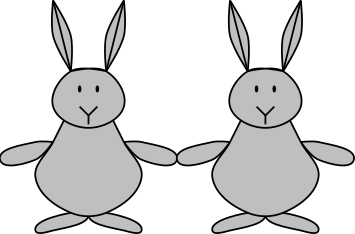
\includegraphics{/home/mattis/projects/graphics/pstricks/rabbits/rabbits.pdf}}\\
#1
\endtabular}

\begin{document}
%\maketitle
\begin{center}
    {\textcolor{Crimson}{\bf \huge  Im Auftrag von GLUE} }
\end{center}

\Table{%
Wir schreiben das Jahr 2020. Sie haben gerade einen neuen Job angenommen und sind nun offizieller
Berater der ``Gesellschaft für Linguistische Unterschiede in Europa" (GLUE). Ihr erster Auftrag
lautet, visuell auf die Unterschiede zwischen den germanischen Sprachen aufmerksam zu machen, und
zwar durch das Erstellen von Alinierungsanalysen von mindestens 100 Wörtern in verschiedensten
germanischen Sprachen. 
 
Zum Glück wissen Sie, dass es einige Sammlungen von Daten zu dem Thema gibt, wie zum Beispiel:
\begin{itemize}
  \item die \textbf{Benchmark Database of Phonetic Alignments}: \url{http://alignments.lingpy.org},
    deren Daten frei von \textbf{Zenodo} (\url{http://dx.doi.org/10.5281/zenodo.11880})
    heruntergeladen werden können (Datei "germanic.zip", darunter wird nur der Ordner "msa"
    gebraucht). 
\end{itemize}

Dort gibt es ja sogar eine germanische Sammlung, die mehr als 100 Dateien umfasst. 

Außerdem kennen Sie mit \textbf{LingPy} (\url{http://lingpy.org}) ja auch eine Bibliothek, mit deren Hilfe phonetische Alinierungen automatisch
durchgeführt und in hübsches HTML-Format überführt werden können. Die Frage ist nur, wie sie einen
möglichst einfachen Workflow erstellen, durch den alle Dateien in einem Gang analysiert werden
können? Da bietet sich natürlich Python an. Außerdem wäre es auch schön, eine Übersicht zu kreieren,
so dass man zwischen den Alinierungen navigieren kann. Hier wäre JavaScript ja praktisch, aber wie
kann man eine HTML-Datei von Python aus erstellen? Sie beschließen, dieses zweite Problem erst mal
beiseite zu legen und sich zunächst um das erste Problem zu kümmern. Falls Sie dann noch Zeit für
das zweite Problem haben, werden Sie sich im Internet Informieren bezüglich der Möglichkeiten, eine
Datei in Python zu erstellen und mit Textinhalt zu füllen. Das dürfte ja eigentlich nicht so schwer
sein...
}

\end{document}

